\documentclass[a4paper,12pt]{article}[abntex2]
\bibliographystyle{abntex2-alf}


% Definições de layout e formatação
\usepackage[a4paper, left=3.0cm, top=3.0cm, bottom=2.0cm, right=2.0cm]{geometry} % Personalização das margens do documento
\usepackage{setspace} % Controle do espaçamento entre linhas
\onehalfspacing % Espaçamento entre linhas de 1,5
\usepackage{indentfirst} % Indentação do primeiro parágrafo das seções
\usepackage{newtxtext} % Substitui a fonte padrão pela Times Roman
\usepackage{titlesec} % Personalização dos títulos de seções
\usepackage{ragged2e} % Melhor controle de justificação do texto
\usepackage[portuguese]{babel} % Adaptação para o português (nomes e hifenização)
\usepackage{multirow}

% Pacotes de cabeçalho, rodapé e títulos
\usepackage{fancyhdr} % Customização de cabeçalhos e rodapés
\setlength{\headheight}{14.49998pt} % Altura do cabeçalho
\pagestyle{fancy}
\fancyhf{} % Limpa cabeçalho e rodapé
\rhead{\thepage} % Página no canto direito do cabeçalho

% Pacotes para tabelas
\usepackage{booktabs} % Melhora a qualidade das tabelas
\usepackage{tabularx} % Permite tabelas com larguras de colunas ajustáveis
\usepackage{float} % Melhor controle sobre o posicionamento de figuras e tabelas

% Pacotes para gráficos e imagens
\usepackage{graphicx} % Suporte para inclusão de imagens

\usepackage[utf8]{inputenc}
\usepackage{listingsutf8}

\lstset{
    language=R,                      
    basicstyle=\ttfamily\scalefont{1.0},
    keywordstyle=\color{blue},       
    stringstyle=\color{red},         
    commentstyle=\color{green},      
    numbers=left,                    
    numberstyle=\tiny\color{gray},   
    stepnumber=1,                    
    numbersep=5pt,                   
    backgroundcolor=\color{lightgray!10}, 
    frame=single,                    
    breaklines=true,                 
    captionpos=b,                    
    keepspaces=true,                 
    showspaces=false,                
    showstringspaces=false,          
    showtabs=false,                  
    tabsize=2,
     literate={á}{{\'a}}1
             {é}{{\'e}}1
             {í}{{\'i}}1
             {ó}{{\'o}}1
             {ú}{{\'u}}1
             {Ú}{{\'U}}1
             {â}{{\^a}}1
             {ê}{{\^e}}1
             {î}{{\^i}}1
             {ô}{{\^o}}1
             {û}{{\^u}}1
             {ã}{{\~a}}1
             {õ}{{\~o}}1
             {ç}{{\c{c}}}1,
}


% Pacotes para unidades e formatação numérica
\usepackage{siunitx} % Tipografia de unidades do Sistema Internacional e formatação de números
\sisetup{
  output-decimal-marker = {,},
  inter-unit-product = \ensuremath{{}\cdot{}},
  per-mode = symbol
}
\DeclareSIUnit{\real}{R\$}
\newcommand{\real}[1]{R\$#1}

% Pacotes para hiperlinks e referências
\usepackage{hyperref} % Suporte a hiperlinks
\usepackage{footnotehyper} % Notas de rodapé clicáveis em combinação com hyperref
\hypersetup{
    colorlinks=true,
    linkcolor=black,
    filecolor=magenta,      
    urlcolor=cyan,
    citecolor=black,        
    pdfborder={0 0 0},
}
\makeatletter
\def\@pdfborder{0 0 0} % Remove a borda dos links
\def\@pdfborderstyle{/S/U/W 1} % Estilo da borda dos links
\makeatother

% Pacotes para texto e outros
\usepackage{lipsum} % Geração de texto dummy 'Lorem Ipsum'
\usepackage[normalem]{ulem} % Permite o uso de diferentes tipos de sublinhados sem alterar o \emph{}

\begin{document}

\begin{titlepage}
    \centering
    \vspace*{1cm}
    \Large\textbf{INSPER – INSTITUTO DE ENSINO E PESQUISA}\\
    \Large ECONOMIA\\
    \vspace{1.5cm}
    \Large\textbf{Atividade Prática Supervionada - APS}\\
    \textbf{Direito e Economia das Políticas Públicas}\\
    \vspace{1.5cm}
    Prof. Luciana Yeung Luk Tai\\
    Prof. Auxiliar  \\
    \vfill
    \normalsize
    Caio Santa Rosa Christovam, \href{mailto:caiosrc@al.insper.edu.br}{caiosrc@al.insper.edu.br}\\
    Érika Kaori Fuzisaka, \href{mailto:erikakf1@al.insper.edu.br}{erikakf1@al.insper.edu.br}\\
    Hicham Munir Tayfour, \href{mailto:hichamt@al.insper.edu.br}{hichamt@al.insper.edu.br}\\
    \vfill
    São Paulo\\
    Maio/2025
\end{titlepage}

\newpage
\tableofcontents
\thispagestyle{empty} % Esse comando remove a numeração de pagina da tabela de conteúdo

\newpage 
\listoffigures
\thispagestyle{empty} % Esse comando remove a numeração de pagina da tabela de figura

\newpage
\setcounter{page}{1} % Inicia a contagem de páginas a partir desta página
\justify
\onehalfspacing

\begin{figure}[H]
    \centering
    \caption{Regras de uso do tobogã}
    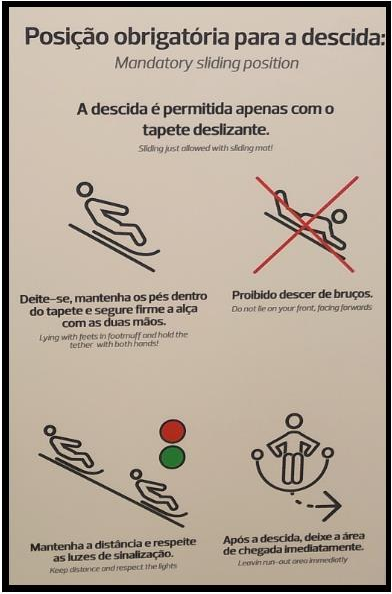
\includegraphics[width=0.75\linewidth]{Imagens/aps1i1.png}
\end{figure}

\textbf{Termos do Contrato}\begin{itemize}
    \item Que as condições de utilização do equipamento visam a proteção da integridade física de todos os possíveis utilizadores do mesmo, de modo que o não cumprimento das condições de segurança pode resultar em danos;

    \item Que estou obrigado a cumprir todas as condições de utilização do equipamento, as quais são requisitos essenciais para minha segurança. O não cumprimento de quaisquer das condições de utilização estipuladas implica na impossibilidade de responsabilização do Insper por quaisquer acidentes ou danos, decorrentes da utilização do equipamento, com o que expressamente concordo e declaro ciência.

    \item Que compreendo a importância da minha conduta para a utilização do equipamento, inclusive para não causar danos a terceiros.
\end{itemize}

\section{\textbf{Cenários}}



\subsection*{{\textbf{INSPER como T.R.E}}}
\subsubsection*{Contexto:}
Durante um princípio de incêndio no prédio, o aluno A opta por usar o tobogã como rota de fuga de emergência, contrariando orientações que restringem seu uso a finalidades recreativas e sob condições normais.

O Insper é a tomadora de risco eficiente, pois tem mais capacidade de prevenir a quebra contratual, seja por meio de sinalização adicional de uso proibido em emergências, bloqueios automáticos, ou treinamento de evacuação mais claro. Logo, a responsabilidade recai sobre B neste cenário.

\subsubsection*{Quebra contratual:}
Uso do tobogã em situação não autorizada e sem supervisão adequada.

\subsubsection*{Barganha hipotética:}
Se ambas as partes soubessem ex ante que haveria um incêndio e o aluno usaria o tobogã como rota de fuga, quem teria maior capacidade de minimizar os danos? O aluno (A) poderia seguir o protocolo de evacuação padrão; já o Insper (B) poderia implementar bloqueios físicos ou instruções claras de que o tobogã não deve ser usado em emergências.

\section*{ALUNO como T.R.E.}

\subsubsection*{Contexto}

O aluno A decide usar o tobogã segurando o celular na mão para gravar um vídeo ou \textit{story}. Durante a descida, o aparelho escorrega, bate nas laterais da estrutura e quebra. Apesar da sinalização de segurança exigir que se use as duas mãos para segurar a alça do tapete e que se evite portar objetos soltos, o aluno acreditou que ``dava tempo'' de descer com o celular.

O aluno é o tomador de risco eficiente, pois estava em posição de evitar o risco com custo praticamente nulo: bastava guardar o celular. A sinalização já estava presente e visível, reforçando a obrigação de descer com as duas mãos na alça. Como o dano decorreu de uma escolha individual, ainda que sem má-fé, a responsabilidade recai sobre A neste caso.

\subsubsection*{Quebra contratual}

Uso do tobogã em desacordo com as normas de segurança, ao portar objeto solto durante a descida, contrariando a orientação explícita de manter as mãos livres e segurar firmemente a alça.

\subsubsection*{Barganha hipotética}

Se ambas as partes soubessem com antecedência que o aluno usaria o celular na descida, quem estaria em melhor posição de evitar a quebra contratual? O Insper poderia, no máximo, colocar um cartaz adicional indicando a proibição do uso de objetos soltos. Já o aluno (A) tinha controle total sobre a ação --- bastava guardar o celular no bolso ou mochila antes de descer.
\newpage
\section{Roteiro}
\subsection*{Abertura do Jornal (1 integrante)}
\textbf{Apresentador(a)}:


 Está no ar o \textit{Quatá News}.\newline
Na edição de hoje, o tobogã do Insper é o centro de duas situações inusitadas que geraram debate jurídico e econômico! \newline
Todos os alunos, ao realizarem a sua matrícula, assinam um contrato sobre o uso do brinquedo.  Esse contrato explicita direitos e deveres das partes — no caso, aluno e escola - para que o tobogã seja usado de maneira segura. \newline
Acontece que recentemente esse acordo foi quebrado em duas situações diferentes e o caso foi parar Justiça. Veja agora na reportagem especial.


\subsection*{Reportagem 1 – Uso em incêndio gera debate (2 integrantes)}

\textbf{Repórter}:
O dia parecia comum no Insper, até que o princípio de um incêndio no prédio 2 levou o aluno \textit{Richard}, a tomar uma atitude desesperada: usar o tobogã como rota de fuga mais rápida.\newline
A decisão, que parece corajosa, contrariava as regras de uso do equipamento e não teve um final feliz - o aluno acabou se machucando devido a alta velocidade e falta do equipamento recomendado para o uso durante a decida do escorregador. \newline

Veja o vídeo do que aconteceu

\textbf{(Corte para imagem do contrato)}
Segundo os termos contratuais, o uso do tobogã está restrito a finalidades recreativas e dentro de condições normais de segurança.\newline

Mas em situação de emergência, quem deveria ter evitado esse uso indevido? Ou, ainda, quem deveria pagar pelos danos ocorridos? O aluno ou a instituição? E para responder essa questão, conversamos com \textit{Paulo Furquim}, especialista em quebras contratuais eficientes.\newline

\textbf{Especialista (Integrante 2):}\newline

Nesse caso temos uma evidente quebra contratual, no entanto, também é verdade que não havia um termo prevendo o que deveria ser feito em caso de incêndio no prédio. Isso acontece devido a um problema fundamental na teoria econômica dos contratos: o fato de que contratos reais não podem ser perfeitamente completos. E o que isso quer dizer na prática? É impossível que um contrato real delineie regras sobre todas as situações relevantes que podem ocorrer. Simplesmente muita coisa pode acontecer e seria custoso demais coloca-las nos termos.\newline

Por esse motivo, sabemos que contratos não devem ser \textbf{\textit{sempre}} aplicados e existe um método que permite identificar o que deveria ocorrer em casos assim. É a famosa barganha hipotética.\newline
Suponha que, antes do incêndio, o aluno e o diretor do Insper tivessem tido a oportunidade de negociar sobre como agir em caso de um acidente como esse. Ambos analisariam quem estaria em melhores condições de evitar o dano e, portanto, quem deveria assumir a responsabilidade caso algo acontecesse. Assumindo uma negociação sem custos, após discutirem custos e possibilidades de prevenção, chegariam à conclusão de que, nesse cenário, a responsabilidade recairia sobre a instituição:  a faculdade teria muito mais condições de assegurar que um incêndio não ocorresse e providenciar medidas de prevenção como bloqueios automáticos ou sinalizações reforçadas para evitar esse tipo de uso inadequado em emergências. \newline 

Portanto, chamamos no caso em questão o Insper de "Tomador de Risco Eficiente", do ponto de vista da teoria econômica dos contratos.\newline


\textbf{Repórter encerra:}
No fim, a responsabilidade recai sobre quem poderia evitar a quebra contratual a menor custo, o tomador de risco eficiente\newline
Bom, depois de fugir do fogo... agora a gente vê o aluno fugindo do bom senso.


\subsection*{Reportagem 2 – Celular na descida: prejuízo ou imprudência? (2 integrantes)}

\textbf{Repórter}:
Você usaria o tobogã segurando o celular só para continuar assistindo os vídeos no tiktok? Foi o que o aluno Richard fez. Mas essa falta de atenção terminou mal: o celular escorregou, bateu nas laterais e se quebrou completamente.\newline

É o que vemos no vídeo a seguir


\textbf{(Corte para imagem da regra de uso)}
A regra é clara: mãos na alça, objetos guardados. Mesmo assim, o aluno se arriscou. E nesse caso, da perspectiva do direito econômico, quem deveria arcar com os danos causados?

\textbf{Especialista (Integrante 4):}
Neste cenário, o aluno é o Tomador de Risco Eficiente. Para determinar isso basta imaginar 
como se daria a barganha hipotética. \newline 

Hipotéticamente, em uma conversa anterior ao incidente, o aluno e o diretor do Insper discutiriam quem teria melhores condições de evitar o dano — e concluíriam que a responsabilidade, nesse caso, caberia ao aluno.\newline

Porque? O aluno tinha controle total da ação e poderia facilmente evitar o dano — bastava guardar o celular. O Insper, por outro lado, poderia fazer o que para evitar a situação? Colocar um funcinário para verificar se os alunos estão cientes das regras? Ou ainda, usar alguma tecnologia avançada para verificar isso? Claramente, soluções muito mais custosas. Como o risco foi assumido individualmente pelo aluno, a responsabilidade de arcar com os danos deveria ser dele. 


\textbf{Repórter encerra:}

Mesmo com sinalização por parte da instituição, o fator decisivo foi a escolha individual do estudante.
Quando a parte que poderia ter evitado o problema decide agir de forma imprudente, o ônus recai sobre ela. Imprudência custa caro — inclusive no mundo jurídico.
E esse é um caso clássico de quebra contratual por um comportamento negligente.\newline

E agora, apresentamos um vídeo de boas práticas feito pelo Insper, a fim de evitar novos acidentes, respeitando todas as regras presentes no contrato.


\subsection*{Encerramento do Jornal (último integrante)}
\textbf{Apresentador(a):}
E assim encerramos a edição de hoje do \textit{Quatá News}. Entre situações inusitadas, aprendemos que os contratos estão em toda parte — inclusive na diversão.

No primeiro caso, o Insper tinha melhores meios para evitar o uso do tobogã em emergência — e falhou. No segundo, o aluno agiu por escolha própria — e arca com as consequências.\newline

Vimos que a lógica do Tomador de Risco Eficiente nos ajuda a atribuir responsabilidade de forma racional: quem pode prevenir o dano com menor custo deve ser o responsável em caso de quebra contratual. Essa análise nos permite dizer como deveria ser feita a aplicação de contratos da melhor forma, com baixa insegurança e mantendo os incentivos das partes alinhadas. Isso contribui para uma maior eficiência econômica dos contratos porque abaixa os custos, tendendo a fomentar mais acordos de ganho mútuo. \newline

Que essas histórias sirvam de alerta e aprendizado. Afinal, entre incêndios e tiktok, entendemos que até o lazer precisa de regras.\newline

O \textit{Quatá News} volta na próxima edição. Boa noite e... reflita antes de escorregar nos contratos. ”

\end{document}